\documentclass[a4paper,10pt]{article}
\usepackage[utf8]{inputenc}
\usepackage{amsmath}
\usepackage{graphicx}
\usepackage{hyperref}
\usepackage{graphicx}

%opening
\title{CS6560 : Assignment 3 }
\author{by CS15B049}
\date{\today}
\begin{document}

\maketitle

\section{OpenMp : }
OpenMP is an Application Program Interface for  shared memory parallel applications.
\subsection{OpenMp constructs used :}
\begin{itemize}
 \item omp\_set\_num\_threads(): the function sets number of threads in the following parallel region.
 \item omp\_set\_nested() : the function enable/disable the nested parallelism.
 
 \item \#pragma omp parallel : Defines a parallel region  that is a block of code that will be executed by multiple threads. it  is the fundamental OpenMP parallel construct.
 
 \item \#pragma omp for : specifies that the iterations of the loop immediately following it must be executed in parallel.
 
 \item Schedule :  Describes how iterations of the loop are divided among the threads in the threads.  \begin{itemize}
                 \item Static : Loop iterations are divided into pieces of size chunk and then statically assigned to threads.
                 
                \item Dynamic : Loop iterations are divided into pieces of size chunk, and dynamically scheduled among the threads, when a thread finishes one chunk, it is dynamically assigned another.
                
                \item Guided : Loop Iterations are dynamically assigned to threads in blocks as threads request them until no blocks remain to be assigned. Similar to Dynamic except that the block size decreases each time a parcel of work is given to a thread.
                \end{itemize}

 
\end{itemize}


\section{Analyzing parallel program performances}
\subsection{Run Time for different Schedule}
Below is the running time of the program A and B under various Schedule type in openmp i.e static, dynamic or guided.\\
N = 100000000\\
Chunk size = N is equally divided among threads.
\subsubsection{For Program A}
\hspace*{5mm} Static :
\begin{center}

\begin{tabular}{ |c|c| } 
 \hline
Thread Number & Time \\ 
 \hline 
 1 &  0.672878\\
  2 & 0.342187 \\
  3  & 0.240974 \\
  4 & 0.216221\\

 \hline
\end{tabular}
\end{center}

Dynamic :
\begin{center}
\begin{tabular}{ |c|c| } 
 \hline
Thread Number & Time \\ 
 \hline 
1 & 0.626382 \\
2 & 0.342168 \\
3 & 0.252023 \\
4 & 0.218553 \\
 \hline
\end{tabular}
\end{center}
\hspace*{5mm}Guided :
\begin{center}
\begin{tabular}{ |c|c| } 
 \hline
Thread Number & Time \\ 
 \hline 
1 & 0.624708 \\
2 & 0.342877 \\
3 & 0.257263 \\
4 & 0.222884 \\
 \hline
\end{tabular}
\end{center}
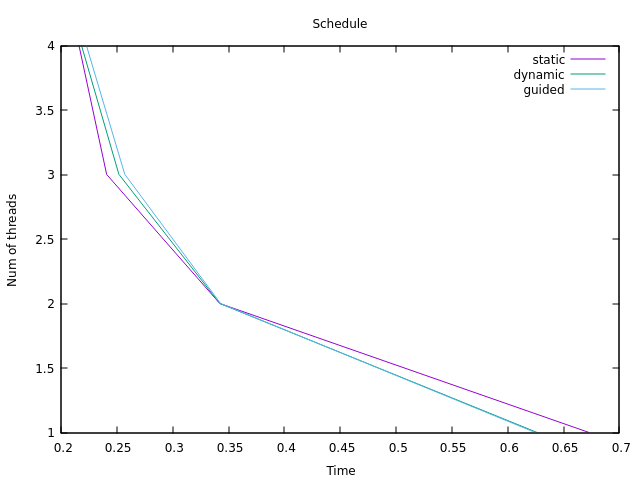
\includegraphics[scale=0.7]{progADiff}\\
GRAPH for Program A
\\
\\
\\
\subsubsection{For program B :}
\hspace*{5mm} Static :
\begin{center}

\begin{tabular}{ |c|c| } 
 \hline
Thread Number & Time \\ 
 \hline 
1 & 0.475659 \\
2 & 0.277407 \\
3 & 0.236133 \\
4 & 0.226071 \\
 \hline
\end{tabular}
\end{center}

Dynamic :
\begin{center}
\begin{tabular}{ |c|c| } 
 \hline
Thread Number & Time \\ 
 \hline 
1 & 0.474254 \\
2 & 0.273875 \\
3 & 0.242267 \\
4 & 0.252879 \\
 \hline
\end{tabular}
\end{center}
\hspace*{5mm}Guided :
\begin{center}
\begin{tabular}{ |c|c| } 
 \hline
Thread Number & Time \\ 
 \hline 
1 & 0.467129 \\
2 & 0.273894 \\
3 & 0.237966 \\
4 & 0.225352 \\
 \hline
\end{tabular}
\end{center}
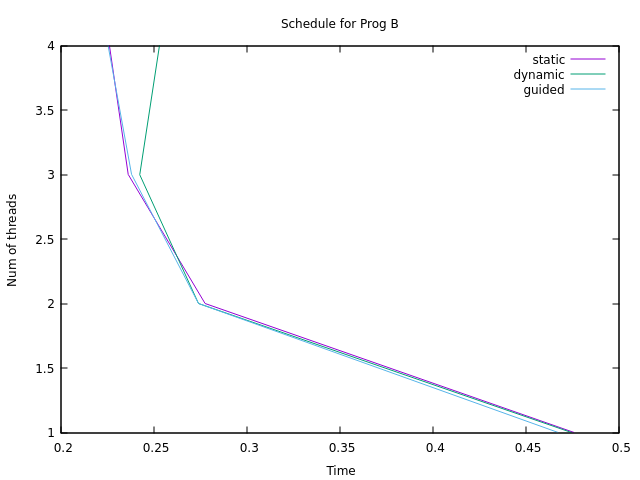
\includegraphics[scale=0.7]{progB}\\
GRAPH for Program B\\
\\
\\
\\
\\
\textbf{Inferences from data:}\\
\begin{itemize}
 \item With increase in number of threads the execution time decreases significantly until a thersold value after which increasing number of threads also increases the execution time.
 
 \item Dynamic vs Static :  for lower number of threads dynamic scheduling does better but as we increase the number of threads the static has lower runtime.
 
 \item Guided is the optimal choice for schedluing as it performs better irrespective of number of threads. 
\end{itemize}


\section{Chunk size vs Time vs Number of Thread}
\subsection{Program A :}
\subsubsection{Dynmaic:}
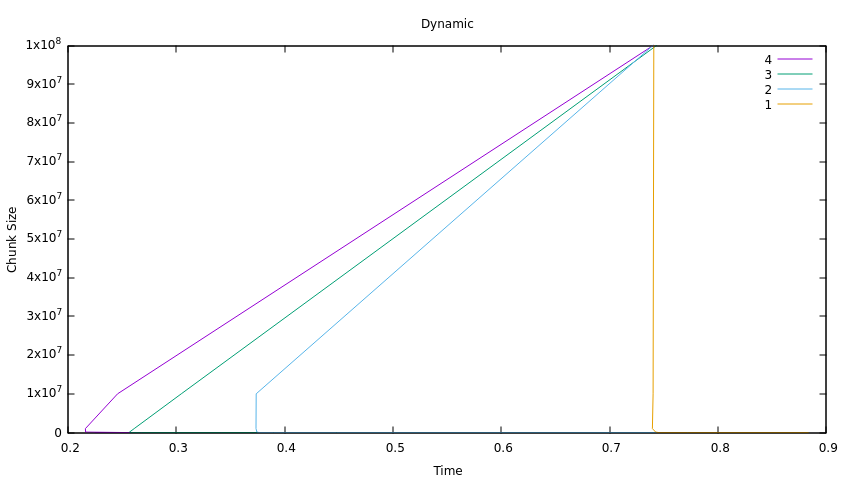
\includegraphics[scale=0.65]{Dynamic}\\
\subsubsection{Static:}
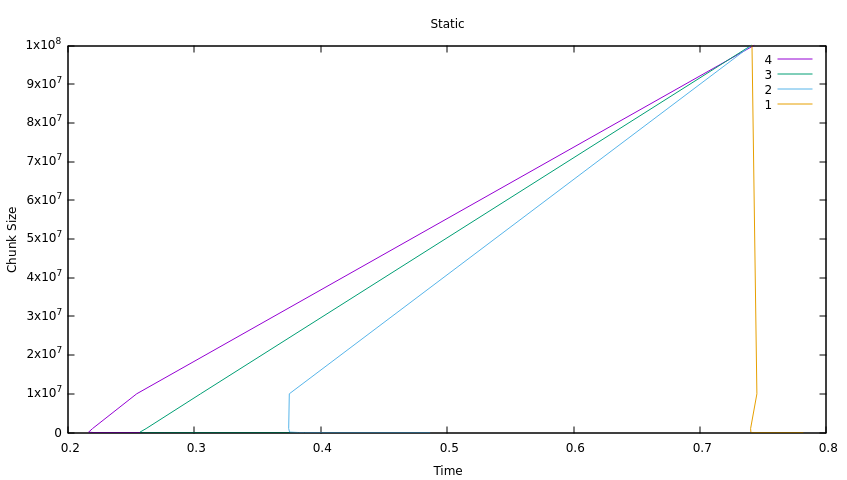
\includegraphics[scale=0.65]{static}\\
\subsubsection{Guided:}
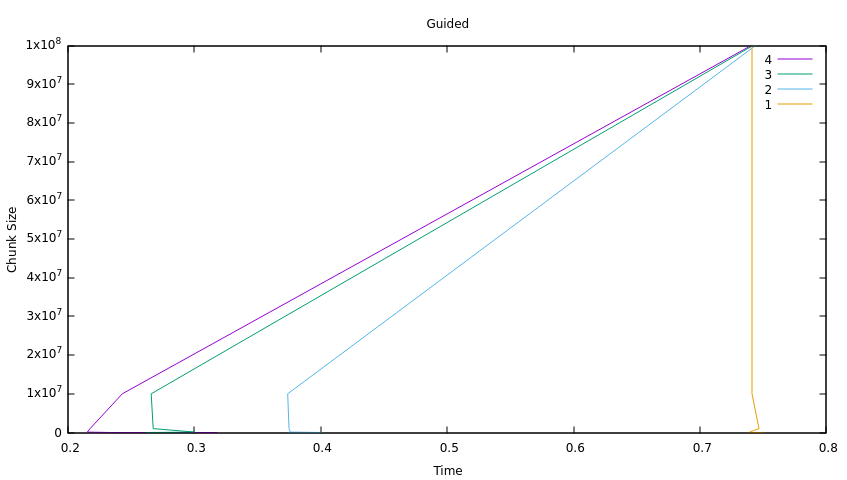
\includegraphics[scale=0.65]{guided}\\
\subsection{Program B :}
\subsubsection{Dynmaic:}
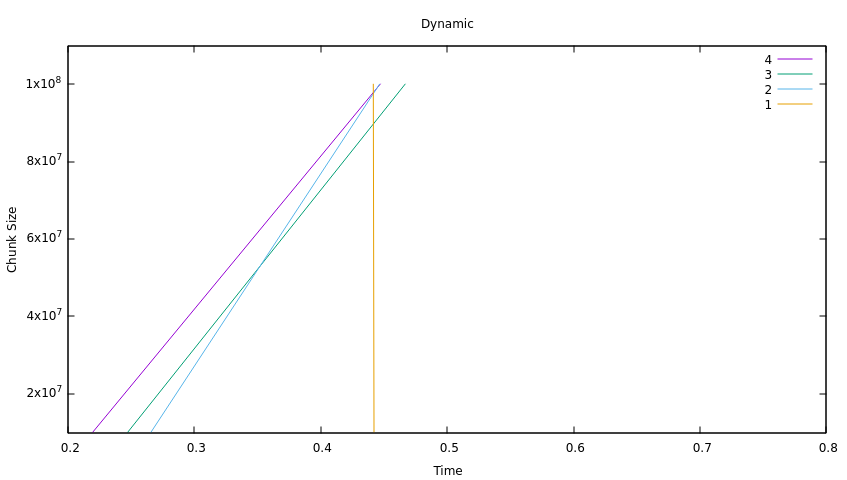
\includegraphics[scale=0.65]{bDyn}\\
\subsubsection{Static:}
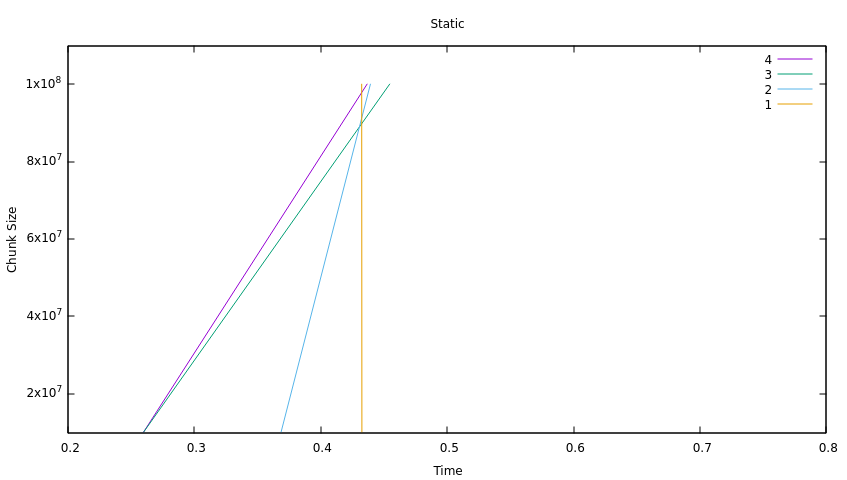
\includegraphics[scale=0.65]{BSTpnd}\\
\subsubsection{Guided:}
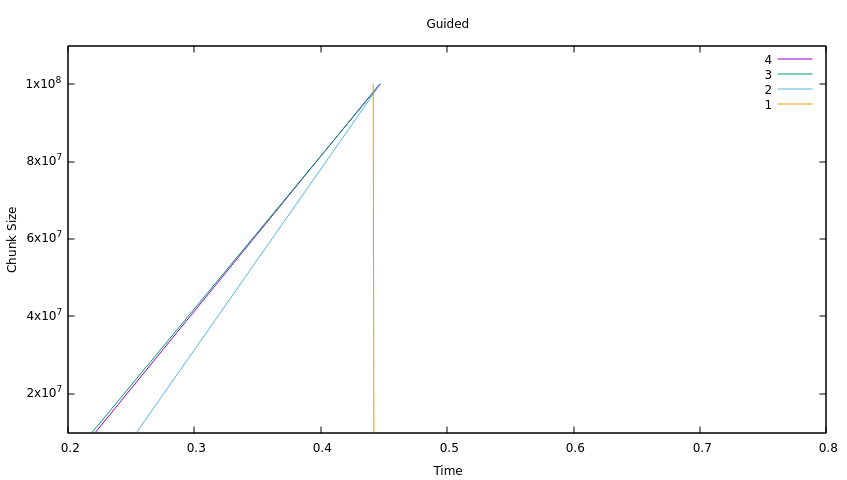
\includegraphics[scale=0.65]{bGT}\\


\end{document}
